\documentclass[tikz, border=10pt]{standalone}
\usepackage{tikz}
\begin{document}
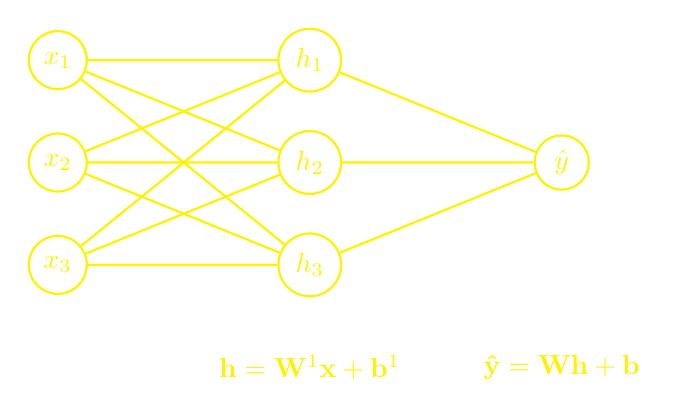
\begin{tikzpicture}[shorten >=0pt, draw=yellow, thick, every node/.style={text=yellow},  xscale=.8, yscale=1.3 ] 
    \tikzstyle{neuron}=[circle, minimum size=12pt, draw=yellow, thick, fill=none]  % Circles with yellow boundary
    \tikzstyle{input neuron}=[neuron];
    \tikzstyle{hidden neuron}=[neuron];
    \tikzstyle{output neuron}=[neuron];
    \tikzstyle{annot} = [text width=4em, text centered]

    % Input layer
    \foreach \x in {1,2,3}
        \node[input neuron] (I-\x) at (0,-\x) {$x_\x$};

    % Hidden layer
    \foreach \x in {1,2,3}
        \node[hidden neuron] (H-\x) at (4,-\x) {$h_\x$};  

    % Hidden layer 1 equation
    \node at (4, -4)  (Hidden1Eq) {
        $\mathbf{h} = \mathbf{W}^1 \mathbf{x} + \mathbf{b}^1$
    };

    % Output layer
    \node[output neuron] (O) at (8,-2) {$\hat y$}; 
    
    % Output layer  equation
    \node at (8, -4 )  (OutputEq) {
        $\mathbf{\hat y} = \mathbf{W} \mathbf{h} + \mathbf{b}$
    };

    % Connect input layer to hidden layer
    \foreach \source in {1,2,3}
        \foreach \dest in {1,2,3}
            \draw (I-\source) -- (H-\dest);

    % Connect hidden layer to output layer
    \foreach \source in {1,2,3}
        \draw (H-\source) -- (O);
\end{tikzpicture}
\end{document}

